%.-------------------------------------------------------------------------------------------------------------------------------------------------------------
\subsection{Overview: High-level component and their interaction}
%.-------------------------------------------------------------------------------------------------------------------------------------------------------------
The SafeStreets App is a distributed App with three logic software layers.
The Presentation layer wich manages the interaction of the user with the system and is responsible of maintaining the GUI, 
the App layer which handles the logic of the App and its functionalities the last layer is the Data access layer which manages the accesses to the database and allows the separation of concerns between business logic and data.
This so called three-tier architecture is thought to be divided on three different hardware layers that represents a group of machines so that every logic layer has a dedicated hardware. This architecture makes it possible to guarantee scalability and flexibility of the system and also lighten the computational load of the server splitting it in two different nodes.
\begin{figure}[H]
\centering
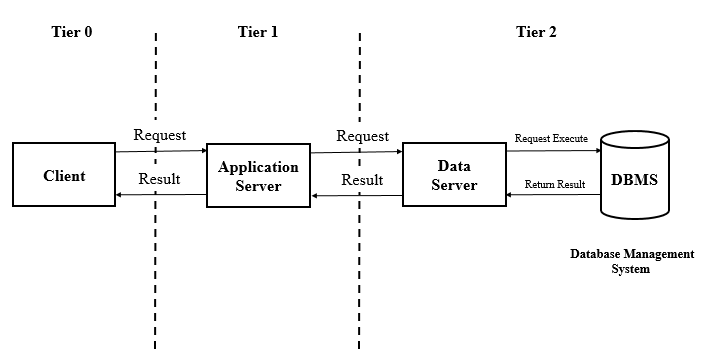
\includegraphics[width=\textwidth]{Images/3tier.png}
\caption{\label{fig:ComWI}Three tier architecture}
\end{figure}
This architecture improves also security of data since users can't access directly data layer but must communicate with App layer that will retrieve only the necessary data.
Citizens accesses the system using their mobile phone App , the App communicates with the App layer to send reports and get statistics , authorities can access the App in the same wway as citizens but they can also receive assignments, see reports and also take on assignments and finish them.
The server of the App layer sends push notifications in asynchronous way to authorities to warn them about violations in the area.
Municipality and System manager communicates with App layer to add new municipality and authorities to the system but also to retrieve statistics and to read suggestions for improving safety on streets.
The App layer communicates with data access layer synchronously to retrieve information and asynchronously to store information about violations.
This kind of architecture allows the server nodes to be replicated to improve the system scalability.
Replicating nodes adds the need for a new component in the architecture , the load balancer, this component is responsible for distributing the working load among the replicated nodes, this Approach also increases the fault tolerance of the service since a fault in a node doesn't affect the service availability. A fault in the system may increase the work load for the other nodes, the number of replications should be decided considering also this possibility to avoid the creation of a bottleneck due to a fault of the server.
To assure security of data managed by the system the server has two firewalls to check packages exchanged with users. Both filters packages incoming and going out of the App logic one towards user devices and the other towards the data access layer.
\newpage
\begin{figure}[H]
\centering
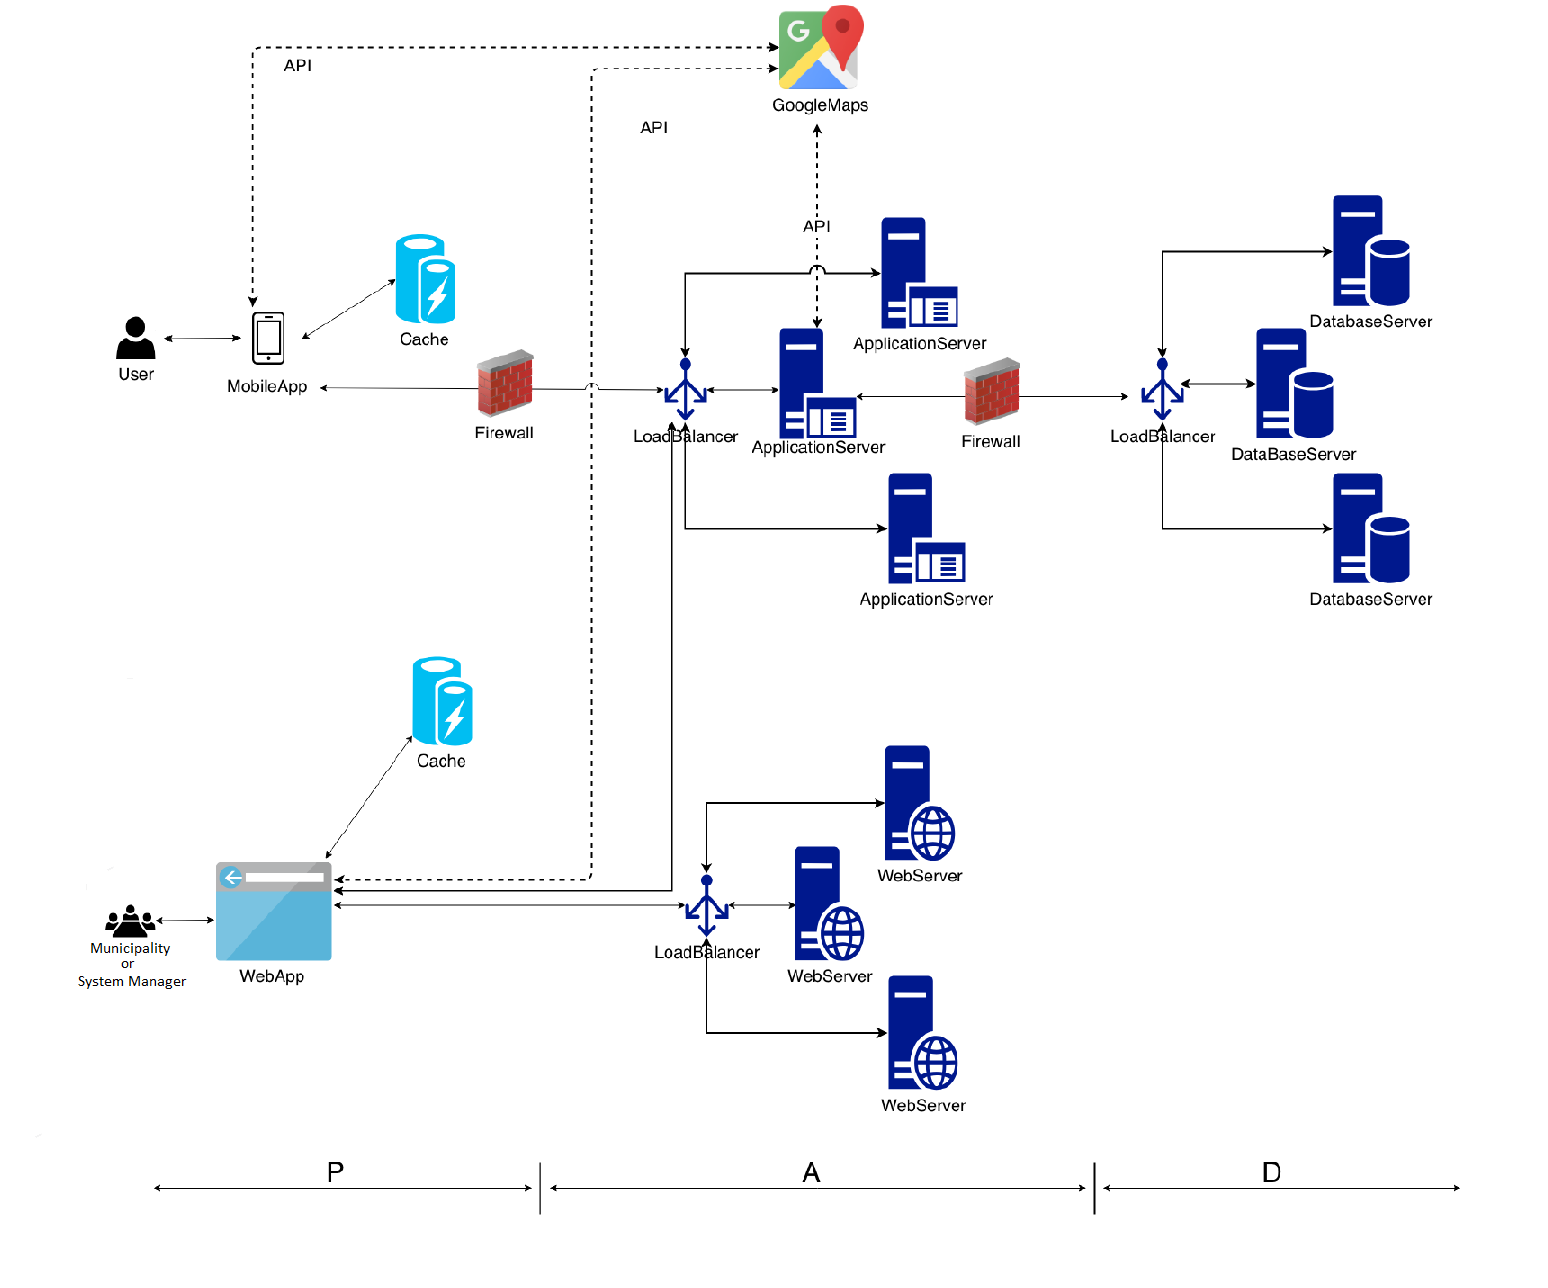
\includegraphics[width=\textwidth]{Images/Architecture.png}
\caption{\label{fig:ComWI}Application High Level Architecture}
\end{figure}
Citizen and authorities are provided of mobile Apps to access the functionalities offered by safestreets. Municipalities and system managers communicates with safestreets using a web App.
The App layer is divided in two parts, one which sends static data (HTML,CSS,Javascript) to web App and another part which communicates with database and provides users dynamic contents.
Our system uses only few caching capabilities because lot of data is dynamic and chages continuosly. The only informations we cache are informations of the violations when an authority takes the corresponding assignment ,citizens have in cache the list of reports they have done and can choose how long that list is kept in memory.
Safestreets uses a relational database to store data about users and violations , the technology used in municipalities' databases depends on the municipality, a different interface may be used to communicate with each of them. For scaling purpouse a non relational database could be used in later releases to collect data from different databases with different structures and then uses mining techniques to find useful information and pattern in recurrent violations and information useful for building statistics may be queried on a regular basis and stored in a location which is faster to access for our system , reducing the number of queries to be done to external databases. 


%TODO change image
%.-------------------------------------------------------------------------------------------------------------------------------------------------------------
\subsection{Component view}
In this section we present the components of SafeStreets we start from a generic point of view showing the main parts which composes our system and then we divide the system in smaller parts to analyse the behaviour of the single components and their subcomponents.
\subsubsection{General Component view}
\begin{figure}[H]
\centering
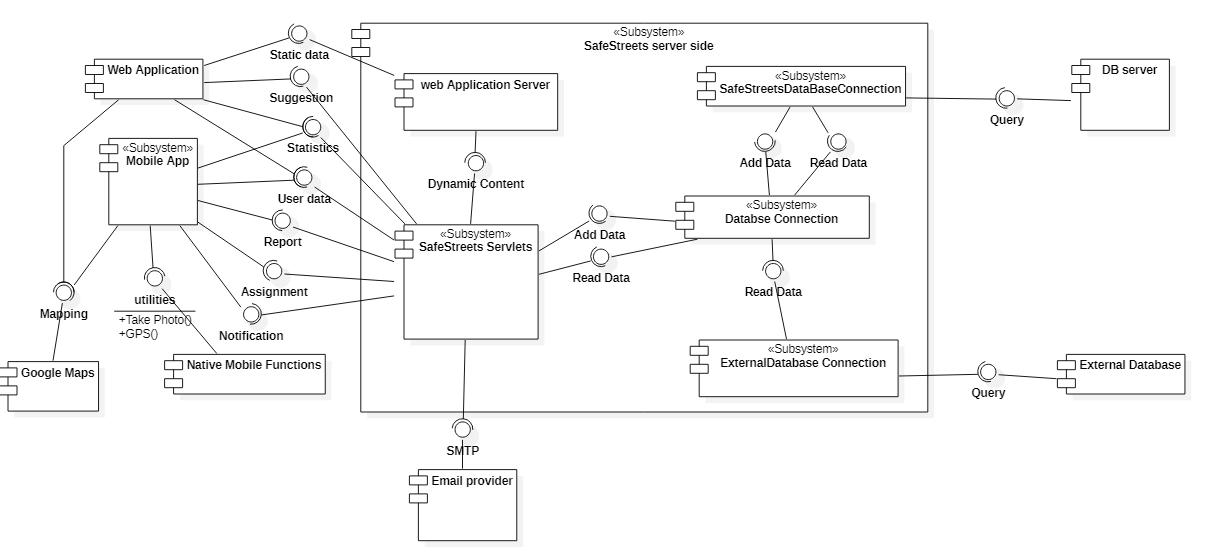
\includegraphics[width=\textwidth]{Images/GenericComponentDiagram.png}
\caption{\label{fig:ComWI}General Component diagram}
\end{figure}
In this diagram we represent a high level logic view on Subsystems and components. We show the interaction between the server and mobile App,web App, email provider and databases.
The server is composed of five SubSystems and components:
\begin{itemize}
\item SafeStreets Servlets: this contains all the Servlets which allows the user to communicate with the server.To retrieve and save data this component communciates with the Database Connection subsystem. All response to the user are sent in JSON format. 
\item Web App Server: this component provides the web App the static data of the App (HTML,CSS,JAVASCRIPT), this part is separated from SafeStreets Servlets for the sake of separation of concerns, dynamic content and static contents are different so different components should get request to retrieve them.
\item DataBase Connection: this component acts as a facade which separates servlets from data access logic. This component communicates with SafeStreets servlets providing them the functionalities to access data.
It communicates to Connection subsystems which communicates with SafeStreets Database and with External Databases to get data which is required by users.
\item SafeStreesDataBaseConnection: this component communicates with SafeStrees database executing query to update and read data from it and provide data to DataBase connection component. 
\item ExternalDatabaseConnection: this component communicates with External databases executing query to read data from it and provide them to DataBase connection component.
\end{itemize}
SafeStreets Servlets communicates using SMTP protocol to send email to users who creates new account or forgets credentials. It also communicates with Mobile App and Web App providing them Access to their acoount data, the possibility to make reports for Citizens , to take assignments for the Authorities, to read suggestions for Municipalities and to see statistics for every type of users and visitors.
The server also communicates with databases to retrieve and save data about violations, users and accidents.
Mobile App and web App both communicates with Google maps API  to get maps to show to users. Mobile App also needs to communicate with functionalities given by the device such as taking Photos and retrieving position using GPS.
\subsubsection{Mobile App and Web App  Component view}
\begin{figure}[H]
\centering
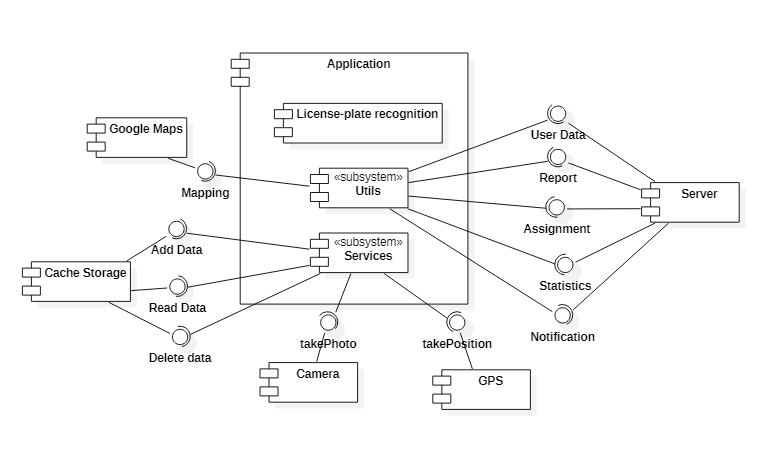
\includegraphics{Images/MobileApplicationComponent.png}
\caption{\label{fig:ComWI} Mobile App Component Diagram}
\end{figure}
In this image we show how Mobile Apllication Subsystem can be seen in more detail.
There are two main components : 
\begin{itemize}
\item Utils:  this component takes care of the communication of the App with SafeStreets Server and Google Maps mApping API.
\item Services: this component communicates with Mobile phone's services which are needed for our App. Those components are GPS which is used to retrieve user position, the phone camera user to take photos of the violations and cache storage used to save locally some useful informations both for Citizens and Authorities.
\end{itemize}
\begin{figure}[H]
\centering
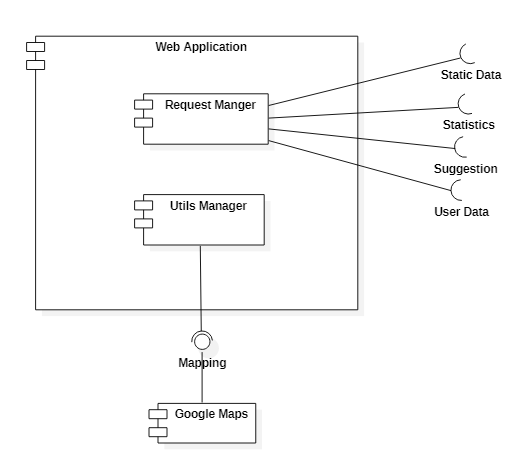
\includegraphics{Images/WebAppComponent.png}
\caption{\label{fig:ComWI}Web App Component Diagram}
\end{figure}
Web App works in a similar way to the mobile App. It must retrieve static data from webServer differently from mobile App.
\subsubsection{Server Servlets Component View}
\begin{figure}[H]
\centering
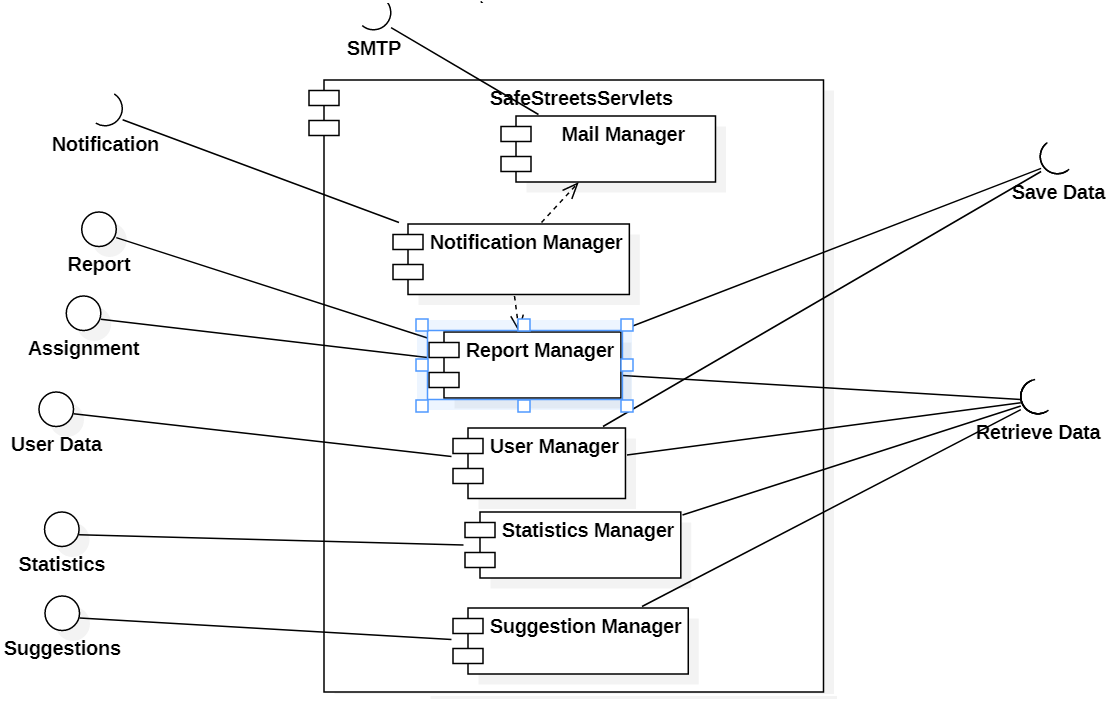
\includegraphics[width=\textwidth]{Images/ServletsComponent.png}
\caption{\label{fig:ComWI} Servlets Compent }
\end{figure}
 SafeStreets Servlets component is composed of 5 Managers:
\begin{itemize}
\item Mail Manager: this component allows the system to send email to Users when they create account or they modify their credentials. This component is associated with user manager which informs it when an account creation or modification is successful.
\item User Manager: this component allows users to create handle their account informations.They can create a new account, modify their data and Login. To allow thees functionalities this component must be able to both save data and retrieve data from database.
\item Report Manager: this component allows citizens to create reports and manage them, and also allows Authorities to take assignments and terminate them. It communicates to the notification manager when new Assignments are created.
\item Notification Manager:This component sends notificiations to authorities about new violations. This component requires that the Mobile App opens a websocket to communicate. 
\item Statistics Manager: This component retrieves data to make  statistics requested by Users and visitors.
\item Sugggestion Manager: This component retrieves suggestion requested by Municipalities.
\end{itemize}
All components takes data and saves data using interfaces exposed by DataBase Connection componet
%.-------------------------------------------------------------------------------------------------------------------------------------------------------------
\subsection{Deployment view}
In the following image the deployment diagram for SafeStreets shows the distribution of the system components and the different deployment nodes. We used a different color to represent External Database servers to show that the node is different, that's because the system should not implement these node but should only communicate with it.
Google Maps API and Email Provider are not shown in this diagram to simplify it and because their interaction with our system are described in component view.
\newline
\begin{figure}[H]
\centering
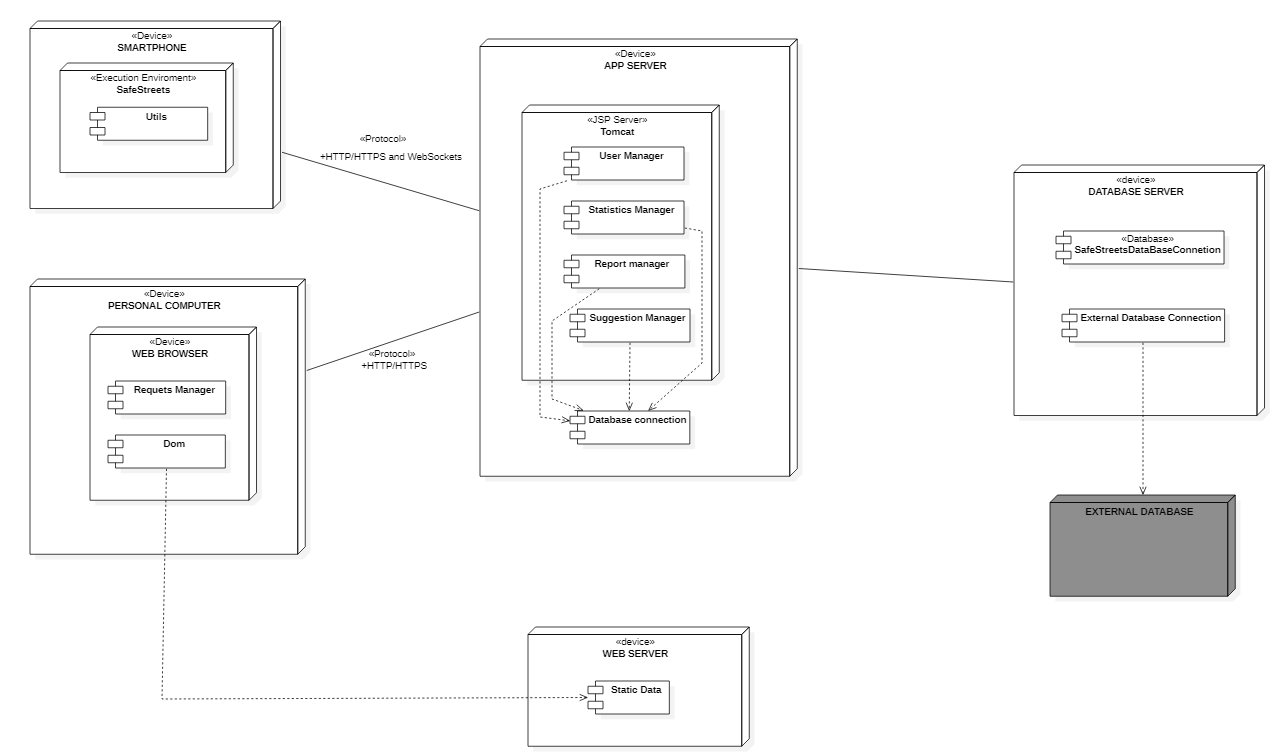
\includegraphics[width=\textwidth]{Images/Deployment.png}
\caption{\label{fig:ComWI} Deployment Diagram}
\end{figure}
This Diagram is divided in three sections to show clearly the separation of the different layers of the App:
\begin{itemize}
\item Presentation : this layer containts the presentation logic. Users to access data must be provided with mobile App for Citizens and Authorities, with web App accessible by a web browser for municipalities and system managers.
Mobile App must be available for both Android and iOS but not just newer versions to make the App the more accessible as possible, for the same reason web App should be compatible with major desktop web Browsers  : Google Chrome, Mozzilla Firefox, Safari and Microsoft Edge(at the time this document is being written).
Communication hAppens using HTTP and HTTPS for both devices while it also hAppens through WebSockets for mobile App push notifications
\item BusinessLogic: this layer is divided in 2 different nodes types. Web Server communicates with webApp and sends it static data needed to render static components(HTML,CSS,Javascript). App Server instead allows users of both type of App to access dynamic data acting as an intermediary to separate presentation and data but also to control access to data.
\item Data Access: This layer excecutes a relational DBMS and provides functionalities to the Business logic to access data requested by users. We show in this layer also the external databases which are another important source of data for SafeStrees.
regarding this component at an initial phase the server will access using the provided interfaces those external databases. When the App will grow a different Approach must be implemented to preserve performances by reducing requests to external systems. To reduce this burden a non relational Database internal to safeStreets may be used to store information from external databases using those as sources to create datamarts and use technologies optimized for Big Data. Using this Approach will add a recurring activity to be performed which is mining this non relational Database to build suggestions for municipalities.
\end{itemize}
%.-------------------------------------------------------------------------------------------------------------------------------------------------------------
\newpage
\subsection{Runtime view}
\subsubsection{Make a report}
\begin{figure}[H]
\centering
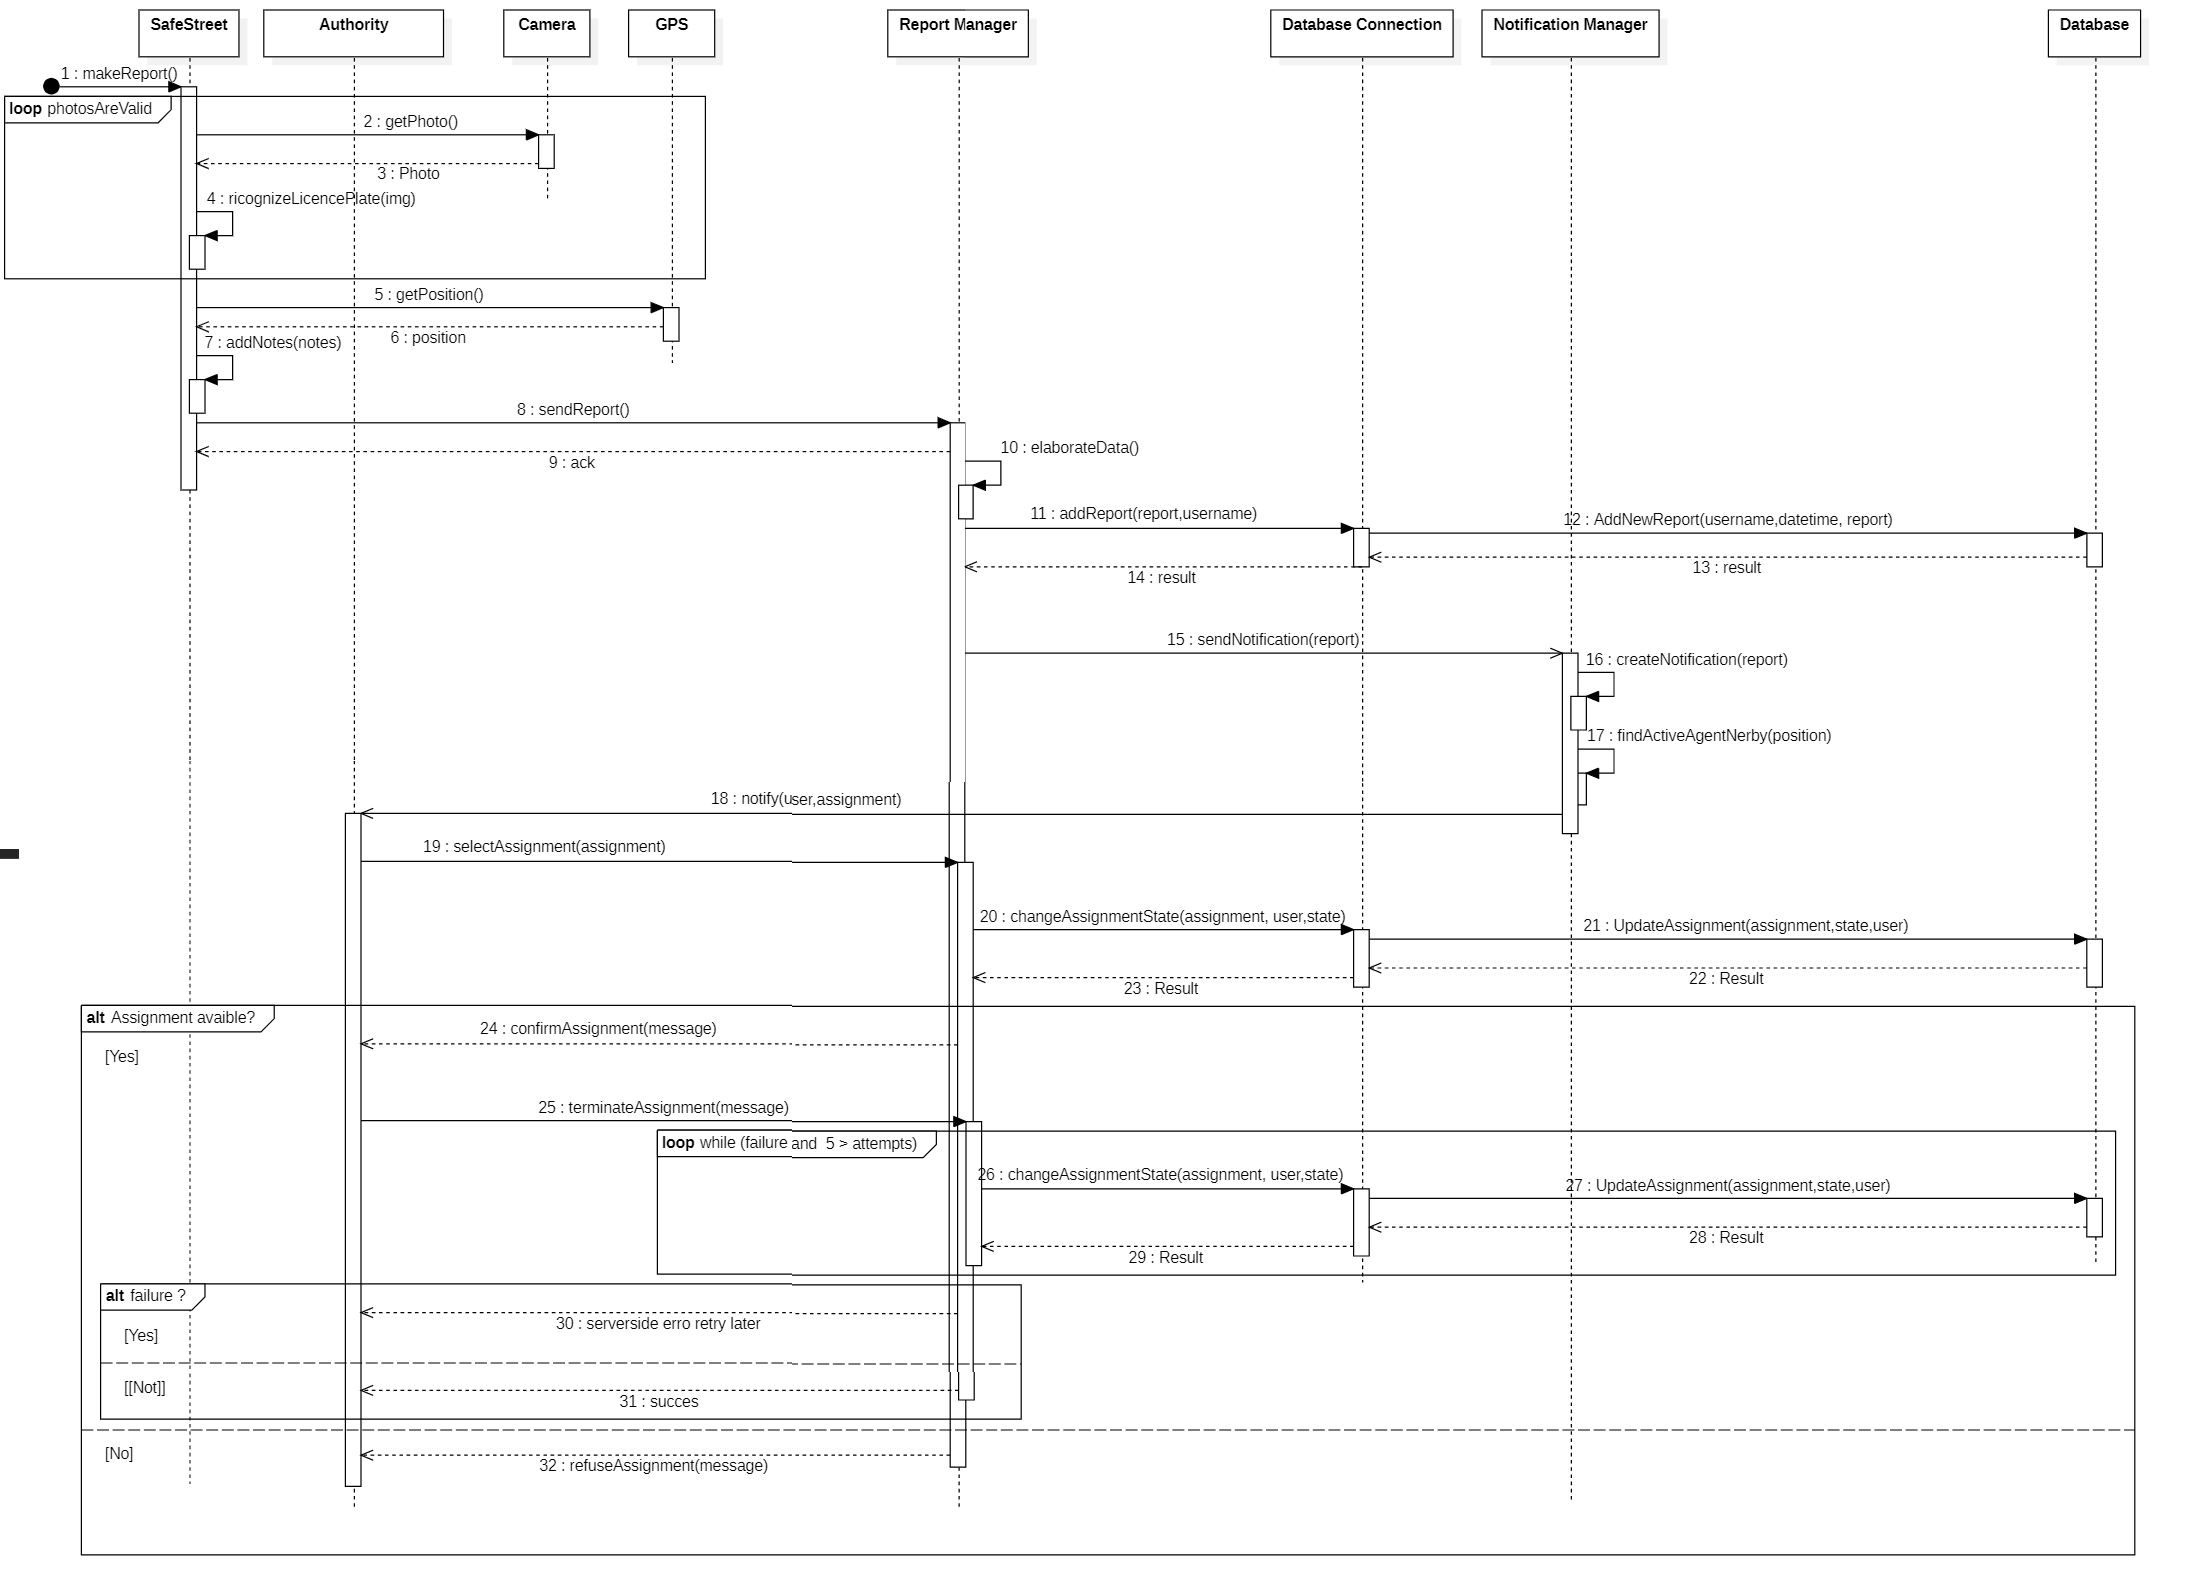
\includegraphics[width=\textwidth]{Images/SequenceMakeReport.png}
\caption{\label{fig:ComWI}Sequence Diagram: Making a Report}
\end{figure}
In this sequence diagram the process through which a Citizen makes a report , the request is handled by server and how the authority is informed and can take the assignment corresponding to the report is shown.
When the Citizen clicks on the Button " Make a Report" of the main creen the phone camera is opened automatically, so user is asked to take the first photo of the violation. After taking the photo it is elaborated with the Algorithm to Recognize Licence Plates if it recognises a licence plate the App gets using the GPS of the App the position of the user , in case of no recognition the user is asked to take another photo. To enrich the Report the App allows the user to write some additional notes that authorities can read and get more information about the violation. Then when the user decides to send the violation clicking on the corresponding button on the UI of the mobile phone the App handles the request and sends the report and all the needed data to the Report Manager.The Report Manager elaborates the data and sends the report to the DatabaseConnection subsystem which takes care to add the report to the DataBase, in this diagram we don't show the SafeStreets database connection subsystem to lighten the diagram and also because it would be called with the same request as the DataBaseConnection resulting in no useful information being added. The Database recognizes if the report is new and creates a new Assignment if it doesn't exist , it just adds a report connected to the assignment if it already exist. After that the Report Manager sends the notification to the notification manager which takes care to find the closest agents to thte report and to warn them using push notifications of the assignment.
The warned authority, who can decide to take the task, in case of acceptance sends a request tot the Report Manager that checks if the Assignment is still available in the database in that case it modifies the state of the assignment and confirms the authority to take charge of the assignment if it was still available otherwise a refusal message is sent to the Authority.
Once the Authority terminates his assignment he can notify the system using the Button "Stop Assignment" after that the App asks the User how the assignment ended and the type of violation. Those data are sent to the Report Manager who modifies the state of the Assignment accordingly If the modification is successful the Report Manager notifies the user otherwise it retries this operation 5 times and than in case of failure it sends an error message to the authority notifing him/her that there are problems in the server and asks the user to retry later to terminate the assignment.
\subsubsection{Login from Mobile App}
\begin{figure}[H]
\centering
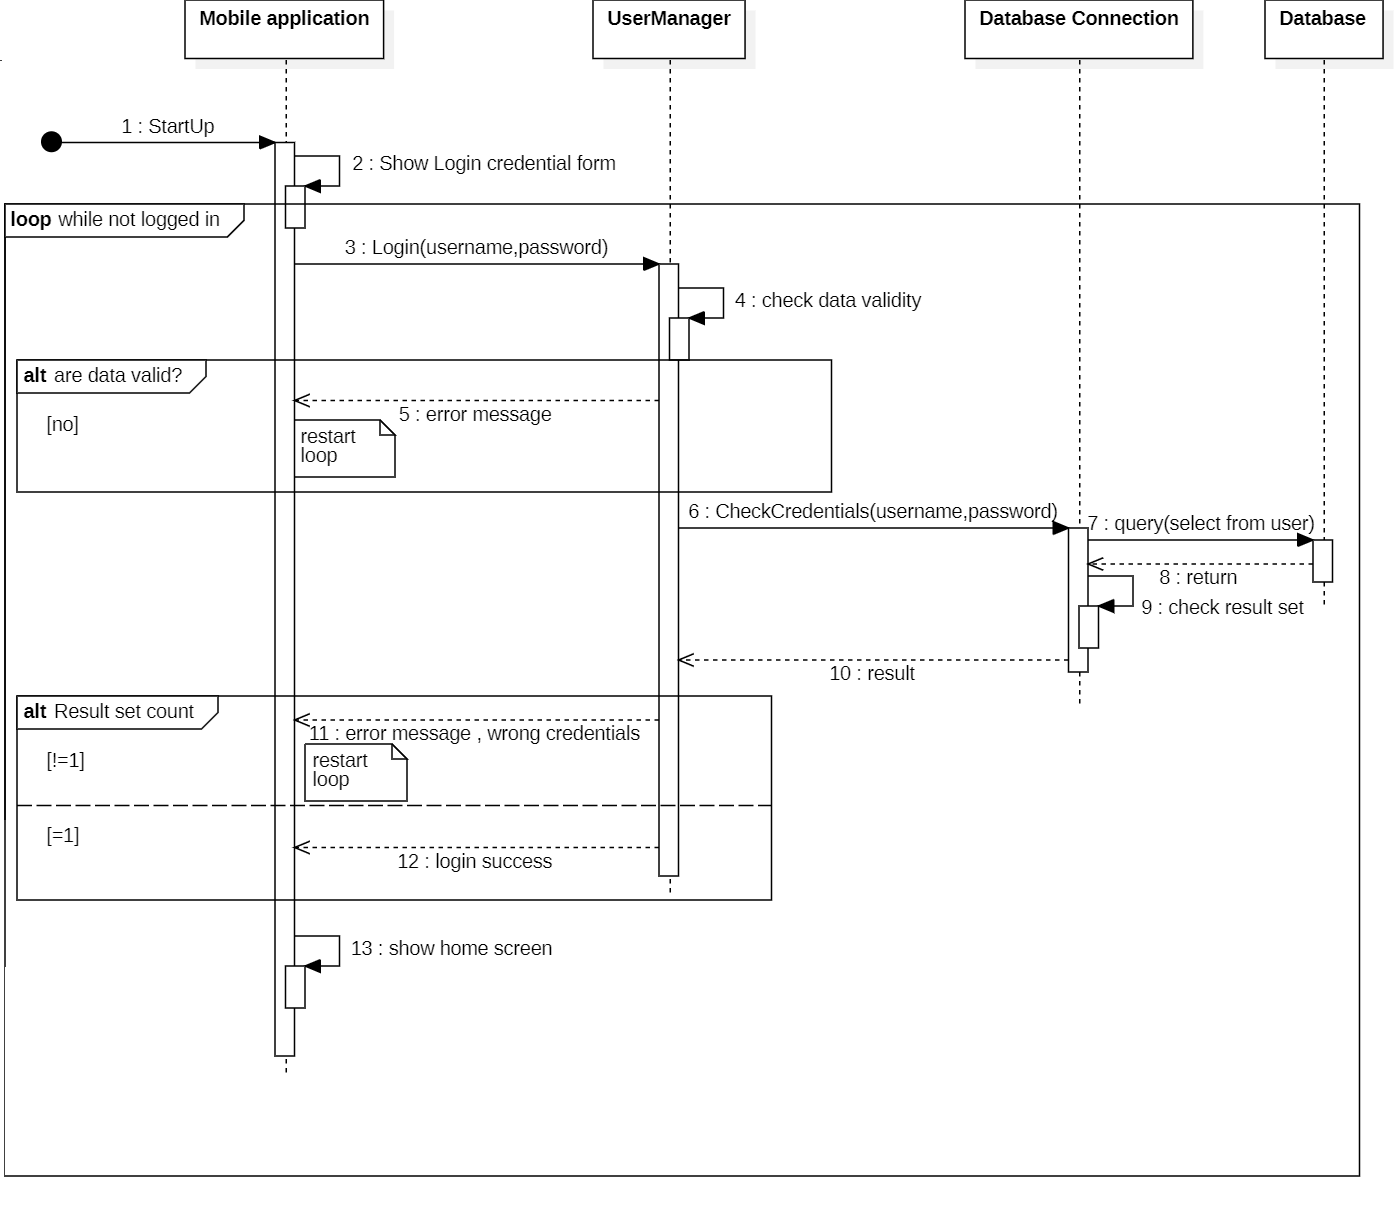
\includegraphics[width=\textwidth]{Images/SequenceLogin.png}
\caption{\label{fig:ComWI}Sequence Diagram: Mobile App Login}
\end{figure}
In this sequence diagram the process through which a User can Login, it shows the Mobile App process but it is the same for the Web App.
Once users gets access to the App(Mobile or Web) they are asked to autenticate themselves in the "Login Page" inserting their credential in the dedicated text fields. Once the user submits the data pressing "Login" button data are sent to User Manager that takes care of the verification of data validity, in case of failure an error message is sent to the user who must repeat the autentication sequence otherwise the User Manager asks the Database Connection subsystem if the credentials are associated with a user also here as in the last diagram the SafeStreets DataBase Connection subsystem is not represented because it wouldn't add relevant interaction for the App. If a  user is found associated to the inserted credential the user is logged in and the homepage is shown to the user otherwise the login request is refused  and the user is notified that the inserted credential are wrong and he/she must retry the Login process.
\subsubsection{Authority registration}
\begin{figure}[H]
\centering
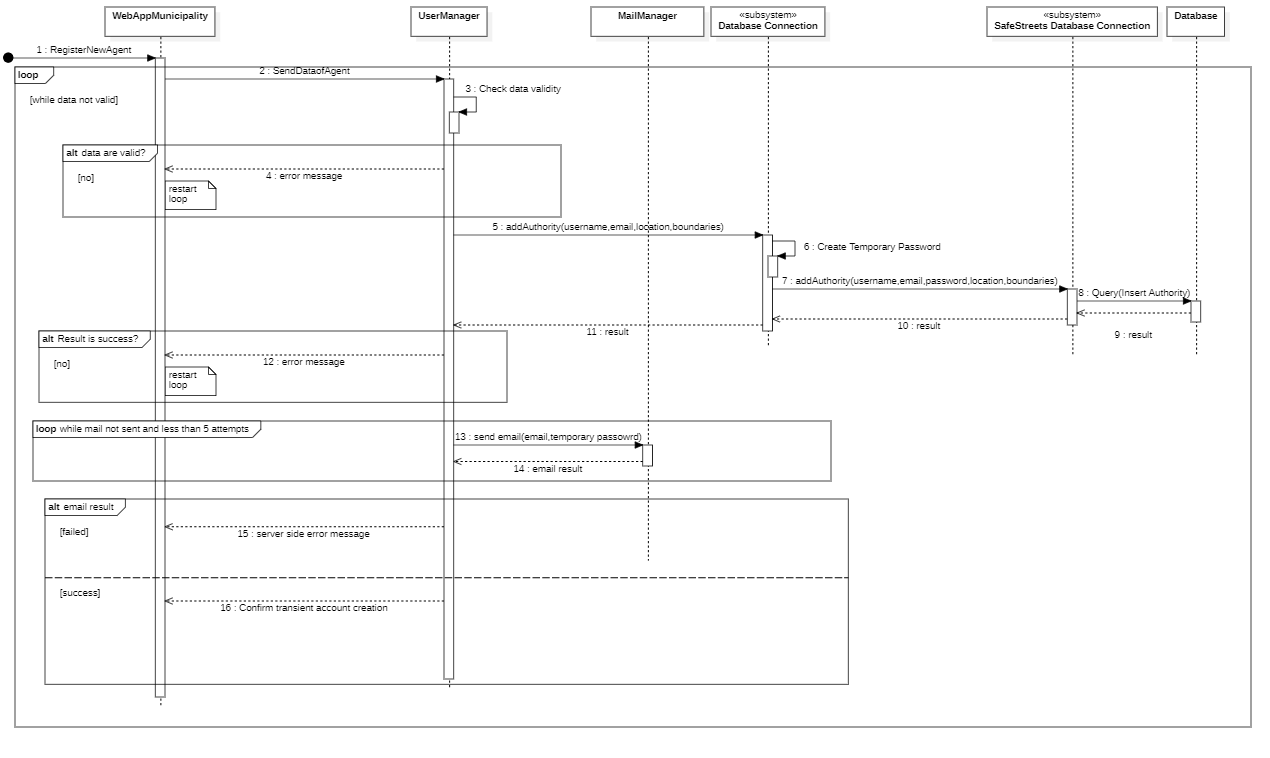
\includegraphics[width=\textwidth]{Images/SequenceAuthorityRegistration.png}
\caption{\label{fig:ComWI}Sequence Diagram :Authority Registration}
\end{figure}
This sequence diagram shows the process of the registration of a new authority to SafeStreets service.
The registration of an authority must be done by a Municipality pressing the "Add Agent" button in the Homepage of Web Application , after this the application shows a page for registrating a new authority , this page contains a form to be compiled with data caracterizing the authority(his/her email adress, username, and the boundaries of the area he/she takes care of). After that the Municipality sends the request to add the agent using the "Add" button, this sends the data from the form to the User Manager which checks if data are valid. In case data are not valid an error message is sent  to the municipality that must refill the form and redo the registration sequence. In case data are valid they are sent to the database conncetion which generates a temporary password for the authority account , after that the SafeStreets Database Connection subsystem checks the existence of an account with the same username. If there is a matching username already in the database the new authority is not registered and the Municipality gets an error message. If the creation is successfull the User Manager asks the Mail Manager to send an email with the temporary password to the Authority . If the email isn't sent and the server fails 5 times to send it, the server informs the Municipality that there are problems with the email and that the server will take care of sending the email if the authority didn't receive an email or in any case if he/she doesn't login within 24 hours. If the email is sent succesfully then authority is informed of the success of the creation of the authority account.
%.-------------------------------------------------------------------------------------------------------------------------------------------------------------
\subsection{Component interfaces}
\begin{figure}[H]
\centering
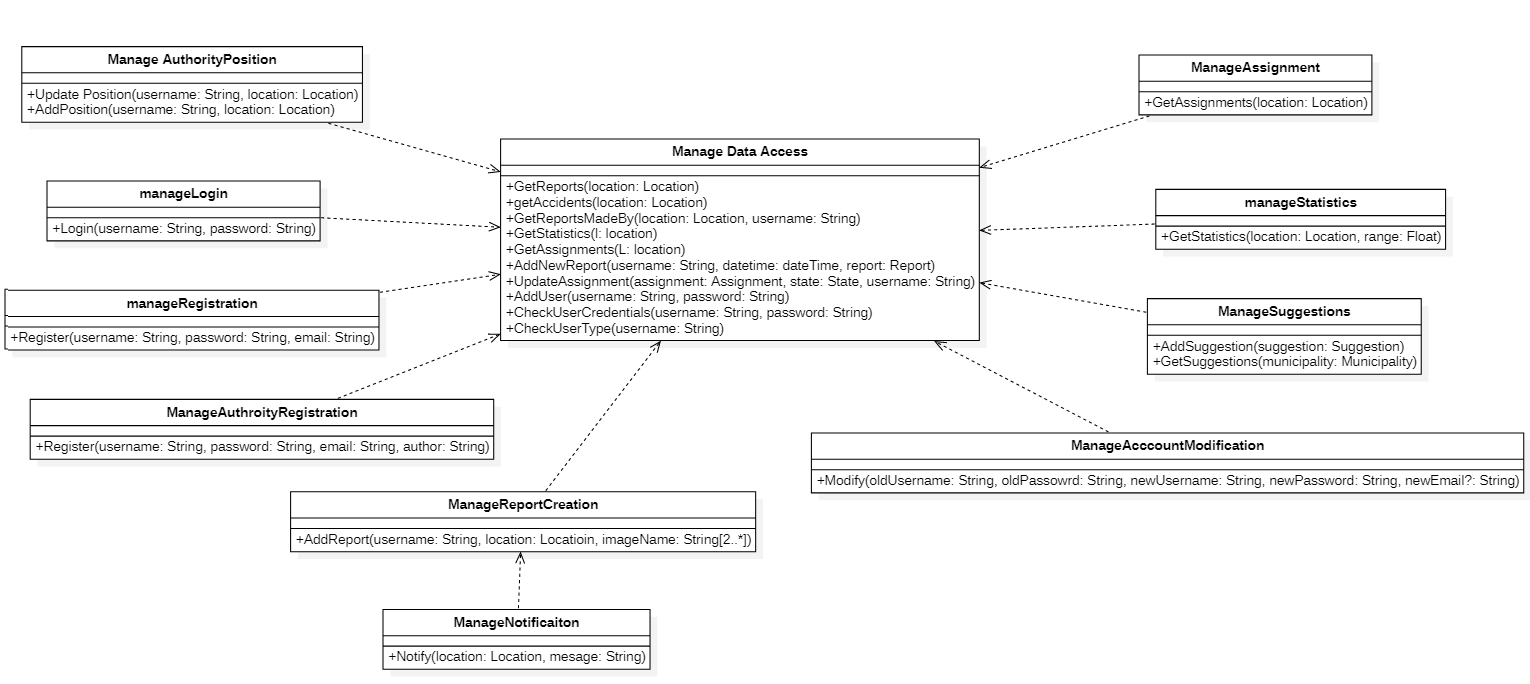
\includegraphics[width=\textwidth]{Images/Interfaces.png}
\caption{\label{fig:ComWI}Component Interfaces}
\end{figure}
In the above picture the component interfaces of the business logic and the facade provided by data access layer are shown.
The arrow represents dependencies between interfaces .
All Interfaces except for ManageDataAccess and ManageNotification are required by the web servlets to respond to user Requests.
Manage Data Acces acts as a facade provided by the Data Connection component and provides the other interfaces the needed data to respond.
Manage Notification takes care of the notification sent to authorities , it need the  Manage Authority Position interface that informs it when an authority moves from one position to another and also it needs the ManageReportCreation  that communicates to ManageDataAccess interface to create a Report object and when the object creation is successful it asks to send notifications to every authority who is active near the location of the report.
Those interfaces are provided by the Manager components of the system:
\begin{itemize}
\item User Manager: provides ManageLogin,ManageRegistration,Manage Authority Position, Manage Authority Registration and Manage Account Modification interfaces
\item Report Manager: provides the ManageReportCreation and manage Assignment interfaces
\item Notification Manager: provides manage Notification interface
\item Statistics Manager:  provides Manage Statistics interface
\item Sugggestion Manager: provides Manage Suggestion interface
\end{itemize}
In this diagram we used the symbol '?' after newEmail in ManageAccountModification to indicate that the old email isn't modified  if it not specified by the user. This difference is done to show how all other parameters must be provided by the Servlets which gets them from users and are mandatory for the functionalities to work.
The most important interfaces needed by servelts to provide user the main functionalities of SafeStreets are:
\begin{itemize}
\item ManageReportCreation: this interface allows the Creation of requests, it needs the username of the user creating it the location of the Violation and the photos associated with it which must be more than 2 [2...n]. It creates an object of type Report and uses the method provided by Manage Data Access to create a new report in case of failure the user is notified, in case of success two different scenarios may hAppen, the report is linked to a new assignment or the report is linked to an already existing assignment, if the already existing assignment is being taken care by an authority the server communicates that to the user who reported the violation in all the other situations the Notification manager is asked to send notification to agents near the location of the violation and are asked to take the assignment.
\item ManageAssignment: this interface allows authorities to find all the pending assignments which are close to their position
\item Manage Suggestions: this interfaces is maily used to allow Municipalities to Get suggestions. Suggestions are made combining Report data and accident data close to the location of the municipality. In addition to dinamically created suggestions Citizens and authorities are able to send suggestions when sending reports for the former or terminating assignments for the latter.
\end{itemize}
\begin{figure}[H]
\centering
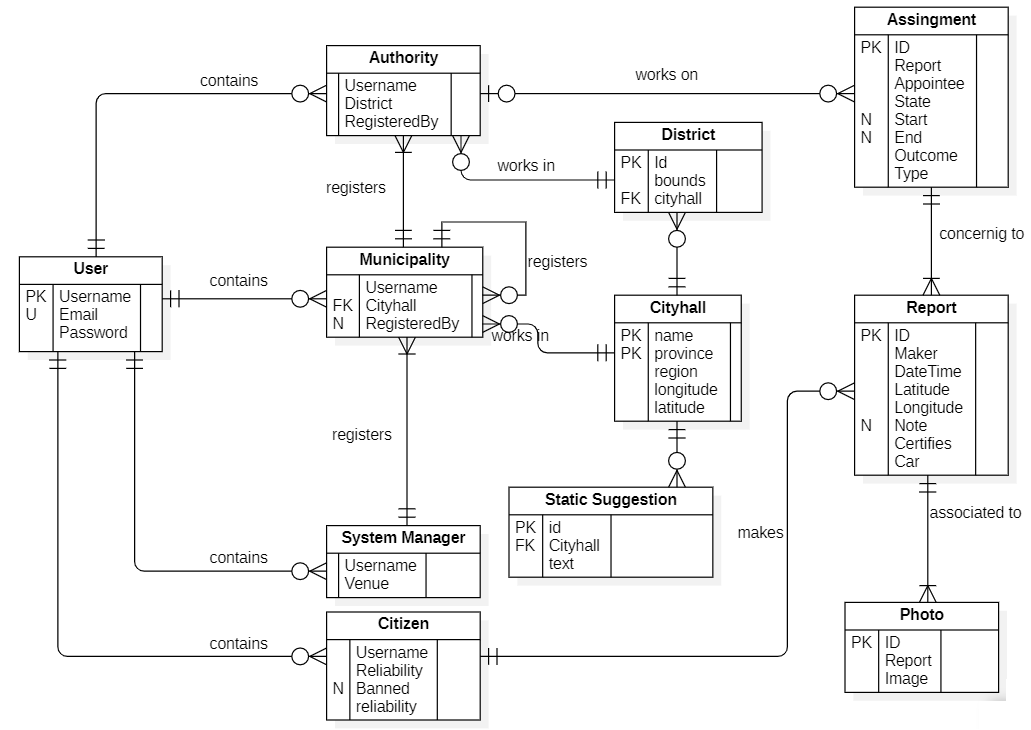
\includegraphics[width=\textwidth]{Images/ER.png}
\caption{\label{fig:ComWI}ER DIAGRAM }
\end{figure}
The image above represents the Entity Relation diagram of data saved on the internal database of SafeStreets. The Different kind of users all have as primary key their username, a unique email is requested for different users because when user account informations gets modified or credential are lost the right user must be notified by eamil. Municipalities have a nullable field RegisteredBy which is used to keep track if an authority registered another authority and who registered them, it can be null if the registration hAppens trough the system manager. To facilitate access to authorities and municipalities in a certain location the cityhall table is used , this table must be indexed using longitude and latitude as indexes to making access to the table faster,
Static Suggestions added by users and authorities must be indexed using Cityhall as an index to make easier access to suggestions.
Report contains a field for notes made by users to authorities to give them information they couldn't provide using photos.
Citizens have a reliability field which represents how reliable a user is , this is used by database to ban a user when they make too many fake reports or they create too many reports in a really short time.
\begin{figure}[H]
\centering
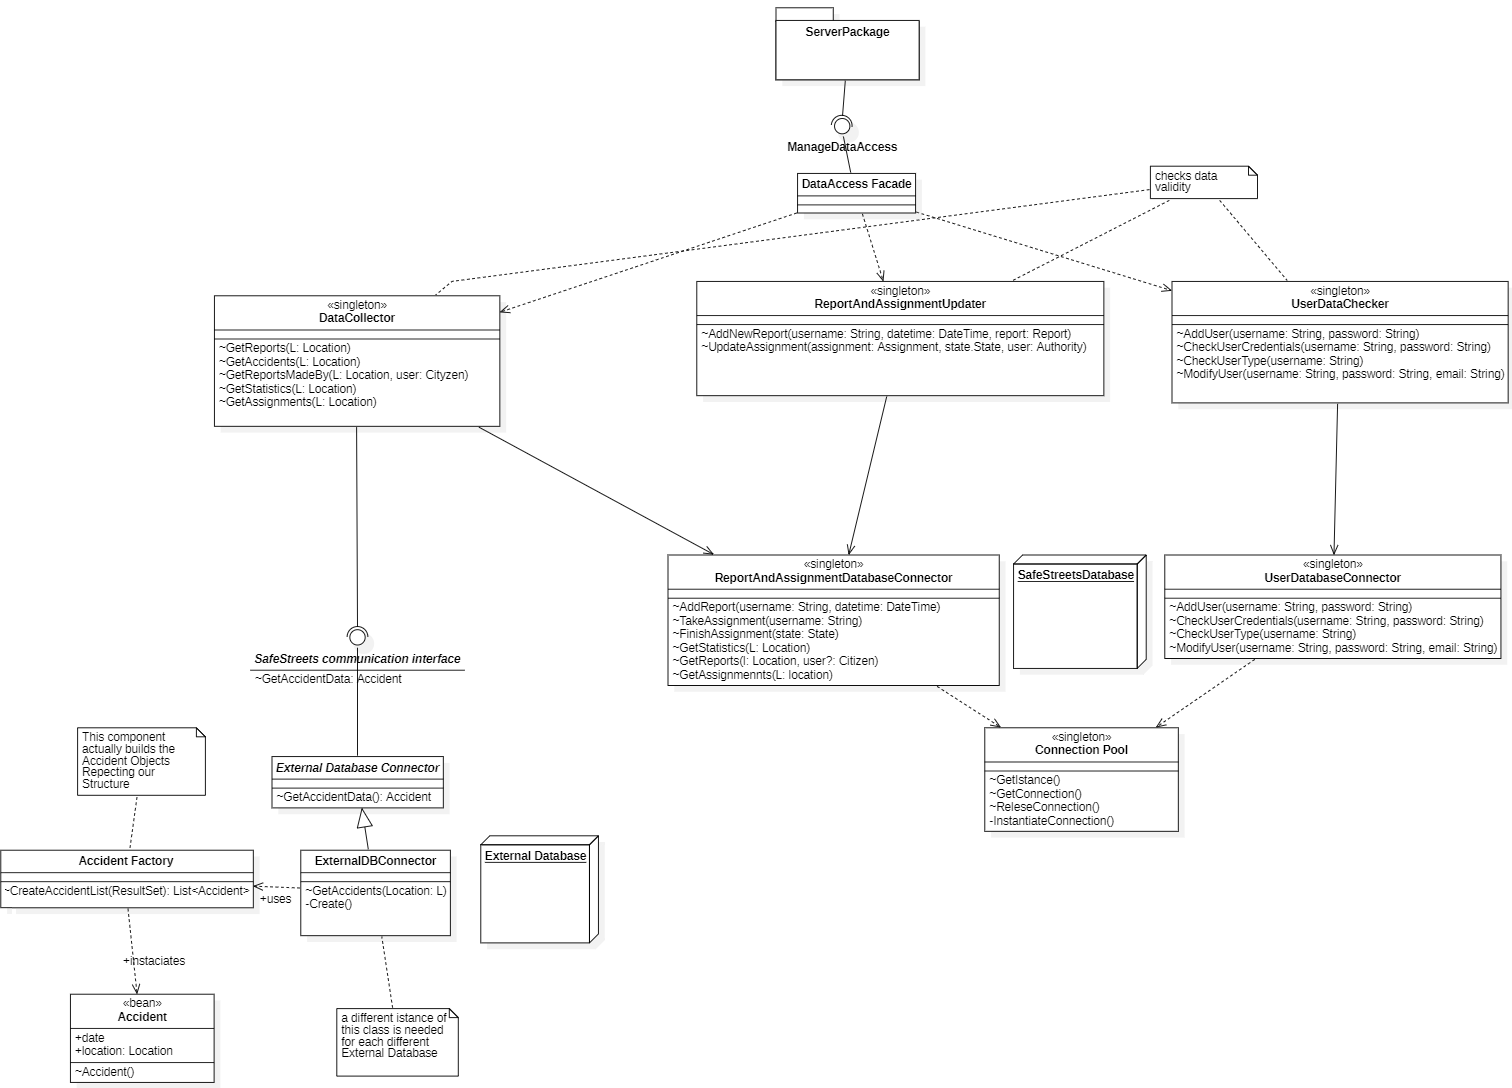
\includegraphics[width=\textwidth]{Images/DatabaseConnectionClassDiagram.png}
\caption{\label{fig:ComWI}Dabase Connection Class Diagram }
\end{figure}
In this picture a part of the class diagram concerning Data Access Layer is provided.
This component provides the Business Logic (here shown as a package, the ServerPackage) an interface to access data.
Internally different singleton classes handles the requests a first group of classes checks input data validity :DataCollector, ReportAndAssignmentUpdater and UserDataChecker. The first one communicates with Report And Assignment Database Connector to get report ,assignment and statistics from SafeStreets Database and also communicates with different External Database Connectors to get Accident data from external Databases. To communicate with external database the system has an abstract class of connector which contains the methods required by the system, for every database a different istance of child class  is needed to implement the actual connection and in case some information need further computation a factory class is needed to create Accident istances which can be used by the business logic. A connection Pool for Connecting to SafeStreets Database to allow the reuse of connection and reduce the cost of memory allocation and disallocation in the server.
 %.-------------------------------------------------------------------------------------------------------------------------------------------------------------
\subsection{Selected architectural styles and patterns}
\subsubsection{Multiple Servlet server}
We choose to use a server which provides multiple servlets to create different access points to the server for different requests. This choice allows us to create separation of concerns SafeStreets Server which is composed of components with few functionalities and a reduced amount of interactions between them. This Approach allows the implementation and testing of components in parallel. The only components which must be developed in advance and tested are Database and database access components. Once those components  are completed  and their functionalities are tested it is possibile to develop different functionalities of the server in parallel, the components must be tested and then integrated with database access components. This Approach allows also to make the system scalable , the different functionalities may be separated in different harware and a routing device may be used to send the request to the right machine which can answer to the request. The system can also be expanded in a really simple way since to add a new functionality a new independent servelt may be added to handle it and then a new manager to handle the request and send it correctly to the database connection components in some cases an  already existing component may be expanded to handle it.
Since different functions of the server are separated in case the system needs to be checked because some functionalities aren't working in the correct way it is possible to pinpoint the parts of the system which aren't correctly working and fix them. For this Approach to work it is really important that the Database access components are working correctly since a bug in that component will affect the overall App making later App maintanance more costly, it is really important that this part is tested in all its functionalities and documentation must be as clear as possible to allow future maintenance and expansions the more simple as possible.
TODO check grammar

\subsubsection{Three Tier Client-Server}

The separation of the system in three different layers allows to makes the system more flexible and reusable.
Together with the multiple Servlet Approach it allows to add functionalities and modifing them without affecing the entire App.
This also allows the separation of the presentation of data to the user from data access using the App layer to block access to informations that a user should not access(I.e. a citizen should not access photos of violations or assignment lists)

%.-------------------------------------------------------------------------------------------------------------------------------------------------------------
\subsection{Other design decisions}
\subsubsection{Thin client }
A thin client is characterized by the fact that it's only function is to communicate with server to retrieve data and concentrates on presentation of data to the user.
\newline
This design choice allows us to separate the business logic from the presentation. However our Mobile App has some business logic in it so it is not purely a thin client. This choice is made to reduce drastically draining computational resources from server. The business logic in the App is the Licence plate recognition algorithm which checks if at least one photo provided by the user contains a valid licence plate, doing such a control server side would have needed to send all the photos to the server to check them and in case of failure notify the App of it and ask the user to re-take photos and send them again to the server, considering also that those kind of algorithm can take lot of time to be executed.
To clarify this statement this example may help to understand our choice: an execution time of a millisecond on a mobile phone may be seen as a bit of lag by the user but if the algorithm runs on the server that millisecond of delay which must be mutiplied by the amount of users sending photos and the number of photos sent by them can result in a delay of seconds in the performances of App server
Nowadays it is important to consider a lot those kind of delay since users can access any kind of App and user experience while using an App is crutial, a delay of just a couple of seconds can make a user uninstall completely an App and also discourage other people from using it.
%---------------------------------------------------------------------------------------------------------------------------------------------------------










